\chapter{Zonal Volume Constraint}
\label{ch:Zonal Volume Constraint}

\begin{figure}[t]
	\centering
	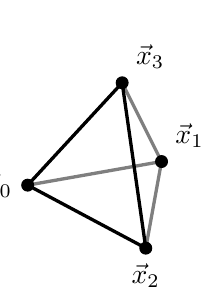
\begin{tikzpicture}
	\useasboundingbox (-1,-1) rectangle (1,2); 
	\draw (-1,0) node[fill, draw, circle ,minimum size=1.5mm,inner sep=0pt,outer sep=0pt, label=left:$\vec{x}_0$](p0){};
	\draw (0.5,-0.8) node[fill, draw, circle ,minimum size=1.5mm,inner sep=0pt,outer sep=0pt, label=south:$\vec{x}_2$](p2){};
	\draw (0.7,0.3) node[fill, draw, circle ,minimum size=1.5mm,inner sep=0pt,outer sep=0pt, label=north east:$\vec{x}_1$](p1){};
	\draw (0.2,1.3) node[fill, draw, circle ,minimum size=1.5mm,inner sep=0pt,outer sep=0pt, label=north east:$\vec{x}_3$](p3){};
	\draw[line width=1.2pt, -] (-1,0) -- (0.5,-0.8);
	\draw[line width=1.2pt, -, opacity=0.5] (-1,0) -- (0.7,0.3);
	\draw[line width=1.2pt, opacity=0.5] (0.5,-0.8) -- (0.7,0.3);
	\draw[line width=1.2pt, -] (-1,0) -- (0.2,1.3);
	\draw[line width=1.2pt] (0.2,1.3) -- (0.5,-0.8);
	\draw[line width=1.2pt, opacity=0.5] (0.2,1.3) -- (0.7,0.3);
	\end{tikzpicture}	
	\caption{A sample tetrahedral element, with 4 vertices at positions $\vec{x}_0$, $\vec{x}_1$, $\vec{x}_2$, and
		$\vec{x}_3$.}
	\label{fig:f2}
\end{figure}

To solve the problem of volumetric locking, instead of enforcing a per-tetrahedron
near-incompressibility with high Poisson's ratio, 
%we propose to enforce incompressibility through constraining volumes of zones defined as local sets of finite elements. Specifically, we add zonal volume constraints to the general energy minimization problem defined in equation~\eqref{eq:energy_min}. 
we adopt the approach of Mixed Finite Element Method as in \ref{eq:mixed_variational}. Essentially,
we solve the saddle-point system as a constrained minimization with constraint function
$\vec{c}(\vec{x}) = \vec{0}$. Specifically, our constraint enforces the total volumes of zones defined as
local sets of finite elements to be preserved.
Compared to other mixed elements, our approach is much more efficient and easier to implement while showing
comparable results. Moreover, our approach provides the modeling flexibility of choosing zones that 
are aligned with anatomical compartments (see Section~\ref{sec:zoning}).

Each constraint is simply formulated as the requirement that the total volume of all elements in a
specified zone of the deformed mesh is equal to the initial volume. That is, for $j$-th zone $G_j$, the zonal
volume constraint function $c_j$ is defined as follows,
\begin{equation}
c_j(\vec{x}) = \sum_{e \in \zeta_j} V_e(\vec{x}) - V_e^0,
\end{equation}
where $V_e^0$ is the reference volume of element $e$, which belongs to zone $j$ with element index set $\zeta_j$.

Imposing this constraint for each zone gives us a new constrained minimization problem:
\begin{align}
\min_{\vec{x}}\ & \int_{\Omega} \Psi(\vec{x}) \\
\text{s.t.}\ & c_j(\vec{x}) = 0 \quad \forall j.
\label{eq:constrained-min}
\end{align}
As a special case we can preserve the total volume with a single \emph{global} constraint; by
contrast, classical incompressible Neo-Hookean models require the volume of each and every element
to be preserved. 

To illustrate the simplicity of this type of constraint we define the volume constraint for a
tetrahedral mesh. The volume of the tetrahedron $e$, as depicted in Figure~\ref{fig:f2}, is defined
(up to a constant scaling) as the triple scalar product
\begin{align*}
V_e(\vec{x}) = \vec{v}_3 \cdot (\vec{v}_1 \times \vec{v}_2),
\end{align*}
where $\vec{v}_i = \vec{x}_i - \vec{x}_0$.  Then the Jacobian of the constraint function can be
computed as
\begin{align*}
\frac{\partial c_j}{\partial \vec{x}} = \sum_{e} \frac{\partial V_e}{\partial \vec{x}},
\end{align*}
where the sparse vector $\frac{\partial V_e}{\partial \vec{x}} \in \R^{3n}$ is zero everywhere
except for the vertices of element $e$, where
\begin{align*}
\left[\frac{\partial V_e}{\partial \vec{x}}\right]_0 = 
-(\vec{v}_2 \times \vec{v}_3 + \vec{v}_3 \times \vec{v}_1 + \vec{v}_1 \times
\vec{v}_2)
\end{align*}\begin{align*}
\left[\frac{\partial V_e}{\partial \vec{x}}\right]_1 = \vec{v}_2 \times \vec{v}_3, \quad
\left[\frac{\partial V_e}{\partial \vec{x}}\right]_2 = \vec{v}_3 \times \vec{v}_1, \quad
\left[\frac{\partial V_e}{\partial \vec{x}}\right]_3 = \vec{v}_1 \times \vec{v}_2.
\end{align*}

%\begin{figure}[t]
%  \centering
%  \begin{subfigure}{.49\linewidth}
%    \centering
%    \includegraphics[width=1.0\textwidth]{images/medpuck_049_50.png}
%    \caption*{(a)}
%    \label{sfig:medpuck_049_50}
%  \end{subfigure}%
%  \begin{subfigure}{.49\linewidth}
%    \centering
%    \includegraphics[width=1.0\textwidth]{images/medpuck_049_vcip_50.png}
%    \caption*{(b)}
%    \label{sfig:medpuck_049_vcip_50}
%  \end{subfigure}\par\medskip
%  \begin{subfigure}{.49\linewidth}
%    \centering
%    \includegraphics[width=1.0\textwidth]{images/puck_049_vcip.png}
%    \caption*{(b)}
%    \label{sfig:puck_049_vcip_50}
%  \end{subfigure}%
%  \begin{subfigure}{.49\linewidth}
%    \centering
%    \includegraphics[width=1.0\textwidth]{images/puck_0475_vcip_50.png}
%    \caption*{(d)}
%    \label{sfig:puck_0475_vcip_50}
%  \end{subfigure}%
%  \caption{\textbf{Reproducing High-Res Simulations}: (a) is a high-resolution puck with 180K
%    tetrahedrons with $\nu = 0.49$ without a zonal volume constraint. (b) is the result with a global
%    volume constraint with the same Poisson's ratio $\nu = 0.49$. (c) shows a low-res simulation
%    with global volume constraint with the Poisson's ratio $\nu = 0.49$, (d) is a lower resolution
%    22K tetrahedrons with our method with $\nu = 0.475$ that recreates the high-resolution results
%    (a) and (b) closely. \todo{remove example and replace with some other case where low-res recreates hi-res}}
%  \label{fig:res_compare}
%\end{figure}
%\todo{fig:res_compare parts c and d. not clear what you are trying to say}
Finally, the Hessian stencils for each $V_e$ will be simple linear skew-symmetric matrices.
% DKP: this needs elaboration that elements are linear in the
% vertex positions. For now, let's save that for another day, since we
% don't exploit it yet.
Thus, $c_{j}(\vec{x}) = 0$ is a one dimensional constraint with simple to implement sparse
derivatives, which gives true volume preservation.
% imcompressibility with respect to the surface of the solid
Note that this constraint can be further optimized by computing the volume of the entire zone by
iterating over zone boundary faces only.

Although uncomplicated, this constraint provides a powerful tool for emulating incompressible
elasticity. It allows users to achieve volume preservation without increasing Poisson's ratio,
which can cause instabilities and locking. For most nonlinear solvers a few equality constraints should not be prohibitively expensive to solve, but for additional performance gain one may naturally use an Augmented Lagrangian method to solve the constraints. 

The zone sizes are important in determining the level of local incompressibility. One global zone
for the entire mesh will essentially be a hydrostatic simulation, analogous to simulating a water
balloon. As the zone sizes decrease, there will be more local incompressibility around each element
which will result in a stiffer behavior. However, as long as the zones are at least as large as the
1-ring \cite{Irving:2007}, volumetric locking will not occur. Therefore, as we use a smaller zone
sizing, the results will become more similar to the results in \cite{Irving:2007}, but at a steeper performance cost. 

Our method can be viewed as a simplification of the 2-field mixed
formulation~\eqref{eq:mixed_variational}, where the pressure potential is given as
\begin{equation}
\vec{p}^{T}\vec{c}(\vec{x}) = \sum_j \vec{p}_j c_j(\vec{x}) = \sum_j \vec{p}_j \left( \sum_{e \in G_j}
V_e(\vec{x}) - V_e^0 \right),
\label{eq:variational_lagrange}
\end{equation}
where the interpolated hydrostatic pressures $\vec{p}_j$ for zone $j$ are identified to be the
Lagrange multipliers for the $j$-th zonal volume constraint. If each element was assigned to a unique
zone, our method would recreate the mixed-element formulation for incompressible materials. However,
we use only a handful of zones, which keeps the problem size small and avoids locking and instability.

\new{
	An important advantage of enforcing volume preservation with zonal constraints is that it allows a way of simulating incompressible
	objects using a much coarser mesh than by using a traditional 1-field method. C\'ea's lemma already couples the quasi-best approximation error 
	with mesh resolution, and since a 1-field FE solutions also couple the bulk modulus to the upper bound of the approximation error, it makes it 
	even harder to use a coarser mesh when bulk modulus is high. However, when incompressibility is decoupled from the bulk modulus, and we can 
	use much smaller $\lambda$, we are able to achieve simulation results of a fine-mesh simulation that is consistent with a much coarser mesh. 
	Figure~\ref{fig:fine-ball} shows a simple dynamic simulation with a very fine mesh, and Figure~\ref{fig:coarse-ball} shows the same simulation
	using a much coarser mesh. We see that both the low Poisson ratio and our method achieves consistent visual results between the fine and coarse
	case, but the high Poisson ratio case fails to converge very early in the simulation.
}

\new{
	We solved the constraints using Ipopt \cite{Wachter:2006}, a non-linear optimization package based on interior point method.
	However, our method should work with any non-linear optimizer that is able to deal with nonlinear equality constraints. 
	In our experiments, we found that not much parameter tuning was required to use our method with Ipopt: we only occasionally had to tune the \texttt{nlp_scaling_max_gradient} parameter when used with additional nonlinear constraints. 
}
\todo{additional explanation on Ipopt?}

\subsection{Stabilization}
We apply the F-bar method \cite{neto:2005} to the energy density function to ensure stability. 
This is based on a multiplicative split of the deformation gradient $\vec{F}$ into 
a deviatoric and volumetric component. The deviatoric part is computed as
\begin{equation}
\bar{\vec{F}}= \alpha \vec{F},
\label{eq:F-bar}
\end{equation}
where
\begin{equation}
\alpha = \frac{\bar{J}^{\frac{1}{3}}}{J^{\frac{1}{3}}},
\label{eq:F-bar_alpha}
\end{equation}
and $\bar{J}$ is the average of $J$ computed over a set of local element stencils. In our case, the
local setss are the zones where the total volume is preserved, hence conveniently 
$\bar{J} = 1$, and $\alpha = J^{-\frac{1}{3}}$. However, since as $J \rightarrow 0$ we have that $\alpha \rightarrow +\inf$, we instead apply a C-2 extension to $\alpha$ below a certain threshold $\epsilon$, similarly to \cite{Stomakhin:2012}. Then the new extended deviatoric projector is given as
\begin{align}
\tilde{\alpha} := 
\begin{cases}
\begin{array}{l} J^{-\frac{1}{3}} \end{array}  & \text{for } J > \epsilon\\
\begin{array}{l@{}l}
\epsilon^{-\frac{1}{3}} &\,-\, \frac{1}{3} \epsilon^{-\frac{4}{3}} (J - \epsilon)
\,+\, \frac{2}{9} \epsilon^{-\frac{7}{3}} (J - \epsilon)^2
\end{array} & \text{for } J \leq \epsilon
\end{cases}
\label{eq:c2}
\end{align}
In practice, the choice of $\epsilon$ is not too important as long as it is small ($\sim 0.1$). 

We then use $\bar{\vec{F}}(\vec{x})$ to compute the deviatoric part of the constitutive equation. For example, 
the deviatoric part of Neo-Hookean energy density function \eqref{eq:neohookean} will now be computed as
\begin{align}
\bar{\Psi}_{\text{NH}}(\vec{\bar{\vec{F}}}; \lambda, \mu) = \frac{\mu}{2}(\tilde{\alpha}^2 I_C - 3).
\label{eq:deviatoric_neohookean}
\end{align}
Note that this is similar to the form presented by \cite{Rivlin:1948}, but extended below 
$\epsilon$ to be continuously defined for $J \leq \epsilon$. 

Using only the deviatoric component of deformation gradient for the elastic potential energy, we remove the contribution of the constitutive equation on the pressure. Hence, this allows the complete split of the total elastic stress, to the deviatoric stress from the elastic potential, and the volumetric stress from the constraint Lagrange multipliers and the volume penalty.